\subsection{\acl{drc}}\label{subsec:drc}

\citeauthor{DRC_2020} propose a method called \ac{drc} 
that faces issues of high intra-class diversities 
due to structural shortcomings in existing deep clustering methods.
They claim that existing methods enforce the representations of samples 
and their augmentations to be assigned to the same cluster,
due to the usage of the maximum sensitivity of the softmax function used during cluster assignment.

\ac{drc} aims to address this issue by considering both the \ac{af} and the \ac{ap} during clustering.
Even though the \ac{ap} can be similar for different samples, their \ac{af} can be different 
as illustrated in \autoref{fig:drc_af_ap}.

\begin{figure}[h] % h = here, t = top, b = bottom, p = page of floats
    \centering
    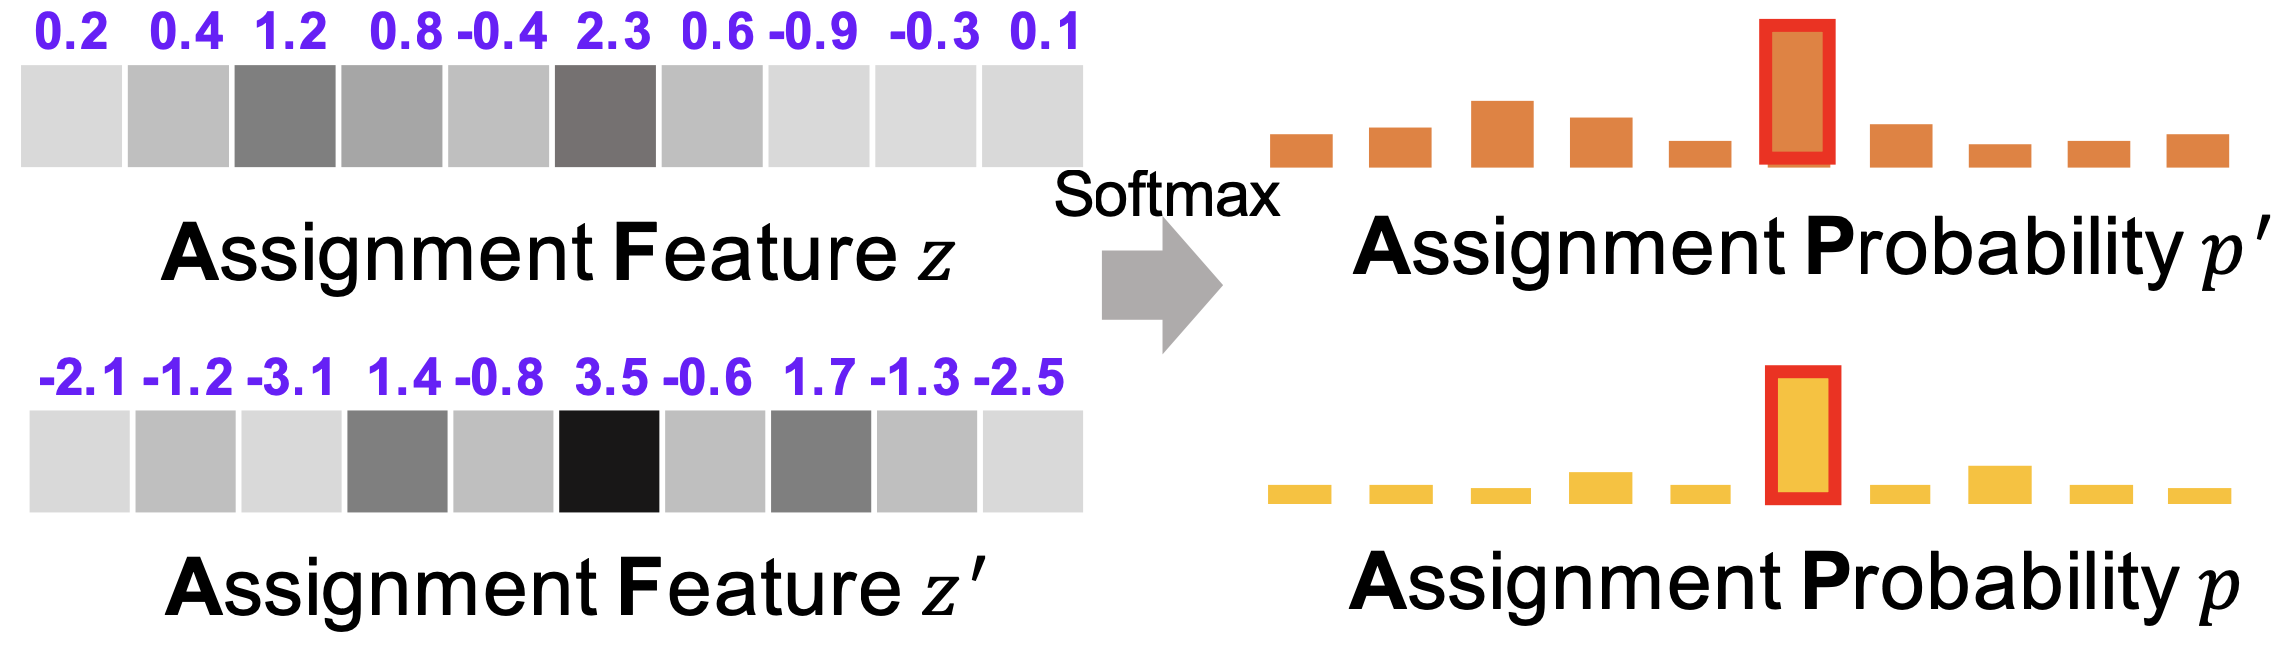
\includegraphics[width=300pt]{images/DRC_af_ap.png}
    \caption{Similar \ac{ap} values for different samples, but different \ac{af} values from \citet{DRC_2020}.
    Cluster assignment based on only \ac{ap} values can result in high intra-cluster diversities.}
    \label{fig:drc_af_ap}
\end{figure}